\documentclass[pdftex,a4paper,11pt]{article} 
%\documentclass[pdftex,a4paper,11pt]{report} 
\usepackage[utf8]{inputenc}
\usepackage[frenchb]{babel}
\usepackage[pdftex]{graphicx}
\usepackage{amsmath}
\usepackage{amssymb}
\usepackage{subfigure}
\usepackage{hyperref}

\hypersetup{
	pdftoolbar=true,                    % show Acrobat’s toolbar ?
	pdfmenubar=true,                    % show Acrobat’s menu ?
	pdffitwindow=true,                  % page fit to window when opened
	pdftitle={Arm model},                    % title
	pdfauthor={Olivier Sigaud},         % author
	pdfsubject={Arm model},                  % subject of the document
	pdfnewwindow=true,                  % links in new window
	pdfkeywords={Arm model},                 % list of keywords
	colorlinks=true,                    % false: boxed links; true: colored links
	linkcolor=black,                    % color of internal links
	citecolor=black,                    % color of links to bibliography
	filecolor=black,                    % color of file links
	urlcolor=black                      % color of external links
}

%\newcommand{\reels}{\mathbb{R}}

\begin{document}

\title{Arm Model}
\author{Thomas Beucher}
\maketitle

\section{Arm model}

The plant is a two degrees-of-freedom (dofs) planar arm controlled by 6 muscles, illustrated in Fig.~\ref{fig:arm_model}.
There are several such models in the literature. The model described in \cite{Kambara2009} lies in the vertical
plane so it takes the gravity force into account. Most other models are defined in the saggital plane and
ignore gravity effects. They all combine a simple two dofs planar rigid-body dynamics model with a 
muscular actuation model. The differences between models mostly lie in the latter component.

\begin{figure*}[hbt]
\centering
	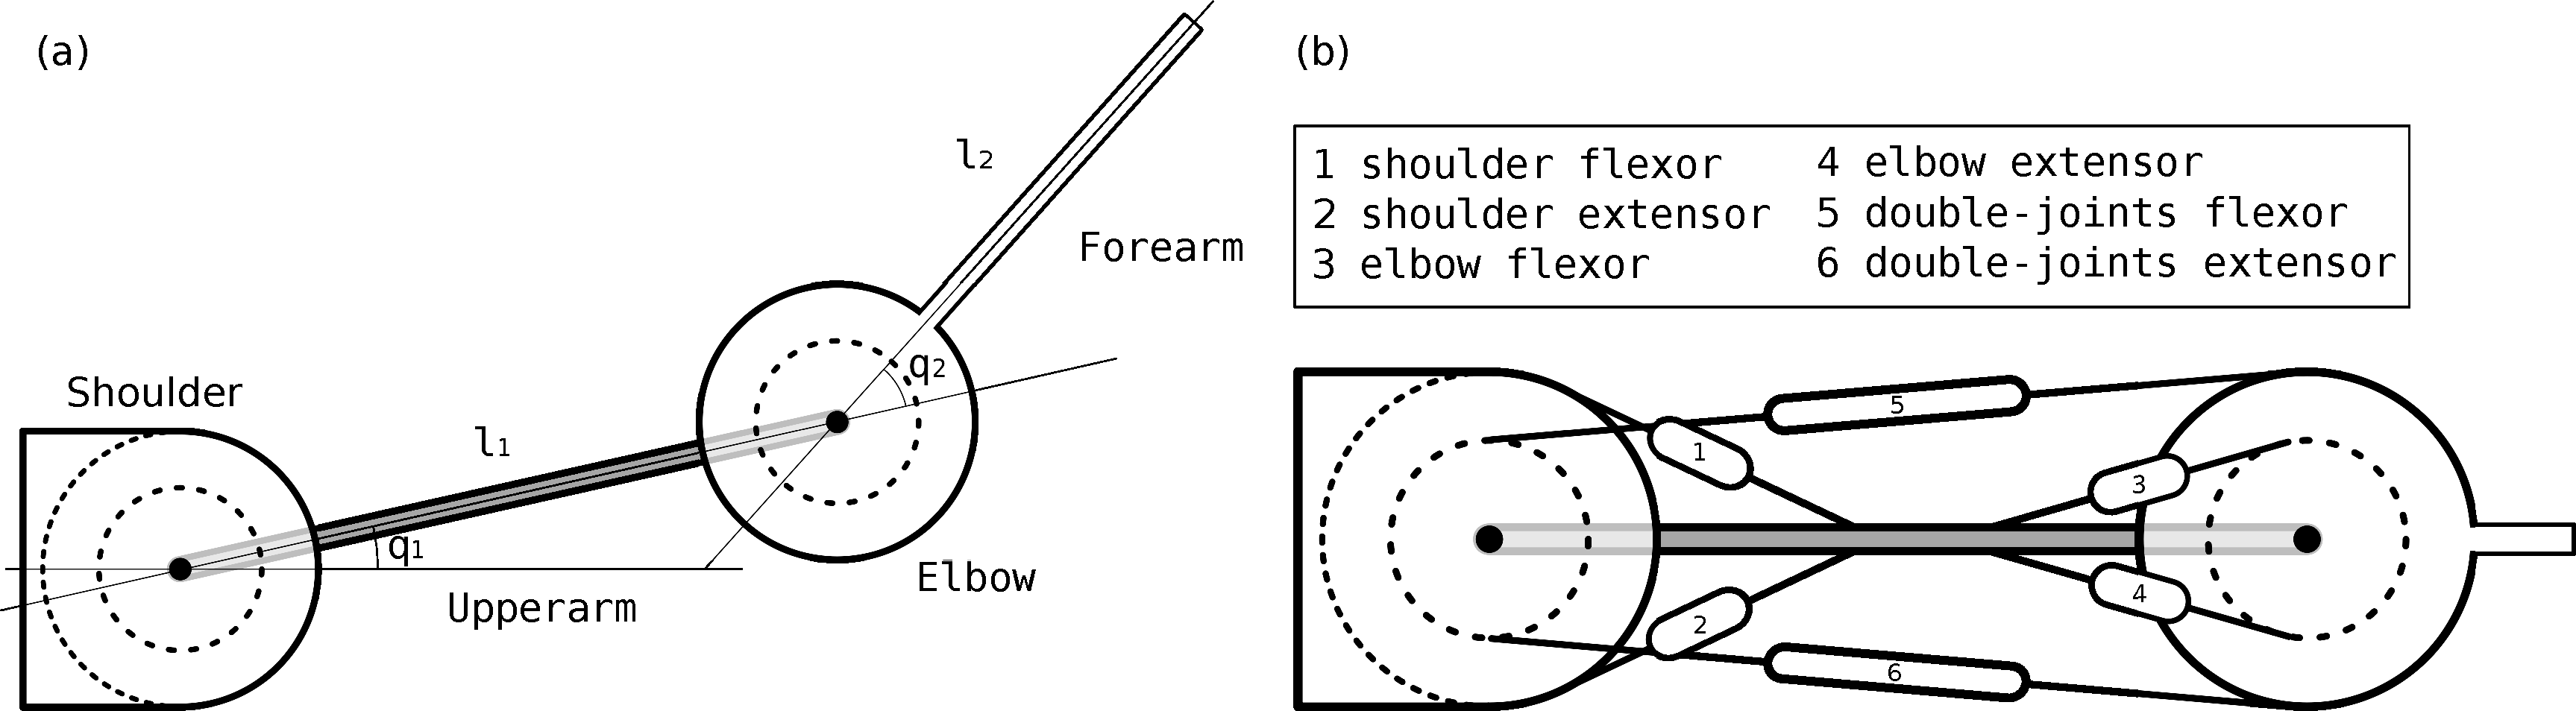
\includegraphics[width=0.9\columnwidth]{figures/arm_model_horiz.pdf}
	\caption{Arm model. (a) Schematic view of the arm mechanics. (b) Schematic view of the muscular actuation of the arm, where each number represents a muscle whose name is in the box.}
	\label{fig:arm_model}
\end{figure*}

Table~\ref{arm_model_params} in Appendix~\ref{sec:params} reminds the nomenclature of all the parameters and variables of the arm model. 

\subsection{Arm parameters}
\label{sec:arm_parameters}
We can find all parameters of the arm in the file \textit{setupArmParameters}.


\appendix
\section{Nomenclature of arm parameters}
\label{sec:params}

\begin{table}[hbt]
\caption{Parameters of the arm model.}
\begin{center}
\begin{tabular}{|c|c|}
\hline  
$m_i$ & mass of segment $i$ ($kg$) \\
$l_i$ & length of segment $i$ ($m$) \\
$s_i$ & inertia of segment $i$ ($kg.m^2$) \\
$d_i$ & distance from the center of \\
      &  segment $i$ to its center of mass ($m$) \\
$\kappa$ & Heaviside filter parameter \\
$\textbf{A}$ & moment arm matrix ($\in \mathbb{R}^{6 \times 2}$)\\
$\textbf{f}_{\textbf{max}}$ & maximum muscular tension ($\in \mathbb{R}^6$)\\
$\textbf{M}$ & inertia matrix ($\in \mathbb{R}^{2 \times 2}$)\\
%$\mat{J}$ & Jacobian matrix \\
$\textbf{C}$ & Coriolis force ($N.m \in \mathbb{R}^2$)\\
$\tau$ & segments torque ($N.m \in \mathbb{R}^2$)\\

$\textbf{B}$ & damping term ($N.m \in \mathbb{R}^2$)\\
$\textbf{u}$ & raw muscular activation (action) ($\in [0,1]^6$)\\
$\sigma_u^2$ & multiplicative muscular noise ($\in [0,1]^6$)\\
$\tilde{u}$ & filtered noisy muscular activation ($\in [0,1]^6$)\\
$\textbf{q}^*$ & target articular position ($rad \in [0,2\pi[^2$)\\
$\textbf{q}$ & current articular position ($rad \in [0,2\pi[^2$)\\
$\dot{q}$ & current articular speed ($rad.s^{-1}$)\\
$\ddot{q}$ & current articular acceleration ($rad.s^{-2}$)\\
\hline
\end{tabular}
\end{center}
\label{arm_model_params}
\end{table}

\begin{table}[hbt]
\caption{Parameters of the arm.}
\begin{center}
\begin{tabular}{|c|c|c|}
\hline  
$\textbf{l}_{\textbf{1}}$ & arm length ($m$) & 0.3\\
$\textbf{l}_{\textbf{2}}$ & forearm length ($m$) & 0.35\\
$\textbf{m}_{\textbf{1}}$ & arm mass ($kg$) & 1.4\\
$\textbf{m}_{\textbf{2}}$ & forearm mass ($kg$) & 1.1\\
$\textbf{s}_{\textbf{1}}$ & arm inertia ($kg.m^2$) & 0.11\\
$\textbf{s}_{\textbf{2}}$ & forearm inertia ($kg.m^2$) & 0.16\\
$\textbf{d}_{\textbf{1}}$ & distance from the center of segment 1 to its center of mass ($m$) & 0.025\\
$\textbf{d}_{\textbf{2}}$ & distance from the center of segment 2 to its center of mass ($m$) & 0.045\\
$\textbf{k}_{\textbf{6}}$ & damping term & 0.05\\
$\textbf{k}_{\textbf{7}}$ & damping term & 0.025\\
$\textbf{k}_{\textbf{8}}$ & damping term & 0.025\\
$\textbf{k}_{\textbf{9}}$ & damping term & 0.05\\
$\textbf{a}_{\textbf{1}}$ & moment arm matrix & 0.04\\
$\textbf{a}_{\textbf{2}}$ & moment arm matrix & -0.04\\
$\textbf{a}_{\textbf{3}}$ & moment arm matrix & 0.0\\
$\textbf{a}_{\textbf{4}}$ & moment arm matrix & 0.0\\
$\textbf{a}_{\textbf{5}}$ & moment arm matrix & 0.028\\
$\textbf{a}_{\textbf{6}}$ & moment arm matrix & -0.035\\
$\textbf{a}_{\textbf{7}}$ & moment arm matrix & 0.0\\
$\textbf{a}_{\textbf{8}}$ & moment arm matrix & 0.0\\
$\textbf{a}_{\textbf{9}}$ & moment arm matrix & 0.025\\
$\textbf{a}_{\textbf{10}}$ & moment arm matrix & -0.025\\
$\textbf{a}_{\textbf{11}}$ & moment arm matrix & 0.028\\
$\textbf{a}_{\textbf{12}}$ & moment arm matrix & -0.035\\
\hline
\end{tabular}
\end{center}
\label{arm_model_params}
\end{table}

\begin{table}[hbt]
\caption{Parameters of the muscles.}
\begin{center}
\begin{tabular}{|c|c|c|}
\hline  
$\textbf{f}_{\textbf{max1}}$ & Maximum force exerted by the shoulder flexor & 700\\
$\textbf{f}_{\textbf{max2}}$ & Maximum force exerted by the shoulder extensor & 382\\
$\textbf{f}_{\textbf{max3}}$ & Maximum force exerted by the elbow flexor & 572\\
$\textbf{f}_{\textbf{max4}}$ & Maximum force exerted by the elbow extensor & 445\\
$\textbf{f}_{\textbf{max5}}$ & Maximum force exerted by the double-joints flexor & 159\\
$\textbf{f}_{\textbf{max6}}$ & Maximum force exerted by the double-joints extensor & 318\\
\hline
\end{tabular}
\end{center}
\label{arm_model_params}
\end{table}

\bibliographystyle{abbrv}
\bibliography{twoDarm}

\end{document}